\chapter{Gaya Antarmolekul dan Pelarut}\label{ch:b1:intermolecular-forces-solvents}

Seekor cicak berlari menaiki kaca jendela dan bergantung padanya dengan
satu jari; tanpa lem, tanpa isapan, hanya tarikan antara molekul-molekul
bantalan jarinya dan molekul-molekul kaca. Air, molekul yang lebih ringan
daripada karbon dioksida, mendidih pada \qty{100}{\celsius}, sedangkan
karbon dioksida berwujud gas pada suhu kamar. Minyak mengapung di atas
cuka dan tidak pernah bercampur dengannya; garam dapur larut dalam air
dan tidak larut dalam bensin. Semua fakta ini ditentukan bukan oleh
ikatan di dalam molekul, melainkan oleh gaya-gaya yang jauh lebih lemah
di antara molekul. Bab ini menggolongkan gaya-gaya itu, mengukur
pengaruhnya terhadap titik didih, dan memakainya untuk memilih pelarut.

% ledger: bp:H2O (the hook's 100 degC)

\begin{recall}
Buku 1 (kelas 11) memperkenalkan gaya van der Waals dan \omterm{def:b1:intermolecular-forces-solvents:hbond}{ikatan hidrogen},
dan menjelaskan bahwa padatan ion larut melalui disosiasi dan \omterm{def:b1:intermolecular-forces-solvents:dissolution}{solvasi}.
\omterm{def:b1:lewis-resonance-vsepr:dipole}{Momen dipol} didefinisikan pada \cref{def:b1:lewis-resonance-vsepr:dipole}
dan \omterm{def:b1:periodicity:polarisability}{polarisabilitas} pada \cref{def:b1:periodicity:polarisability}. Dari
fisika kita memakai hukum Coulomb: dua muatan $q_1$ dan $q_2$ yang
berjarak $r$ di vakum saling tarik atau saling tolak dengan gaya yang
normanya $|q_1q_2|/(4\pi
\varepsilon_0 r^2)$.
\end{recall}

\begin{omfigure}
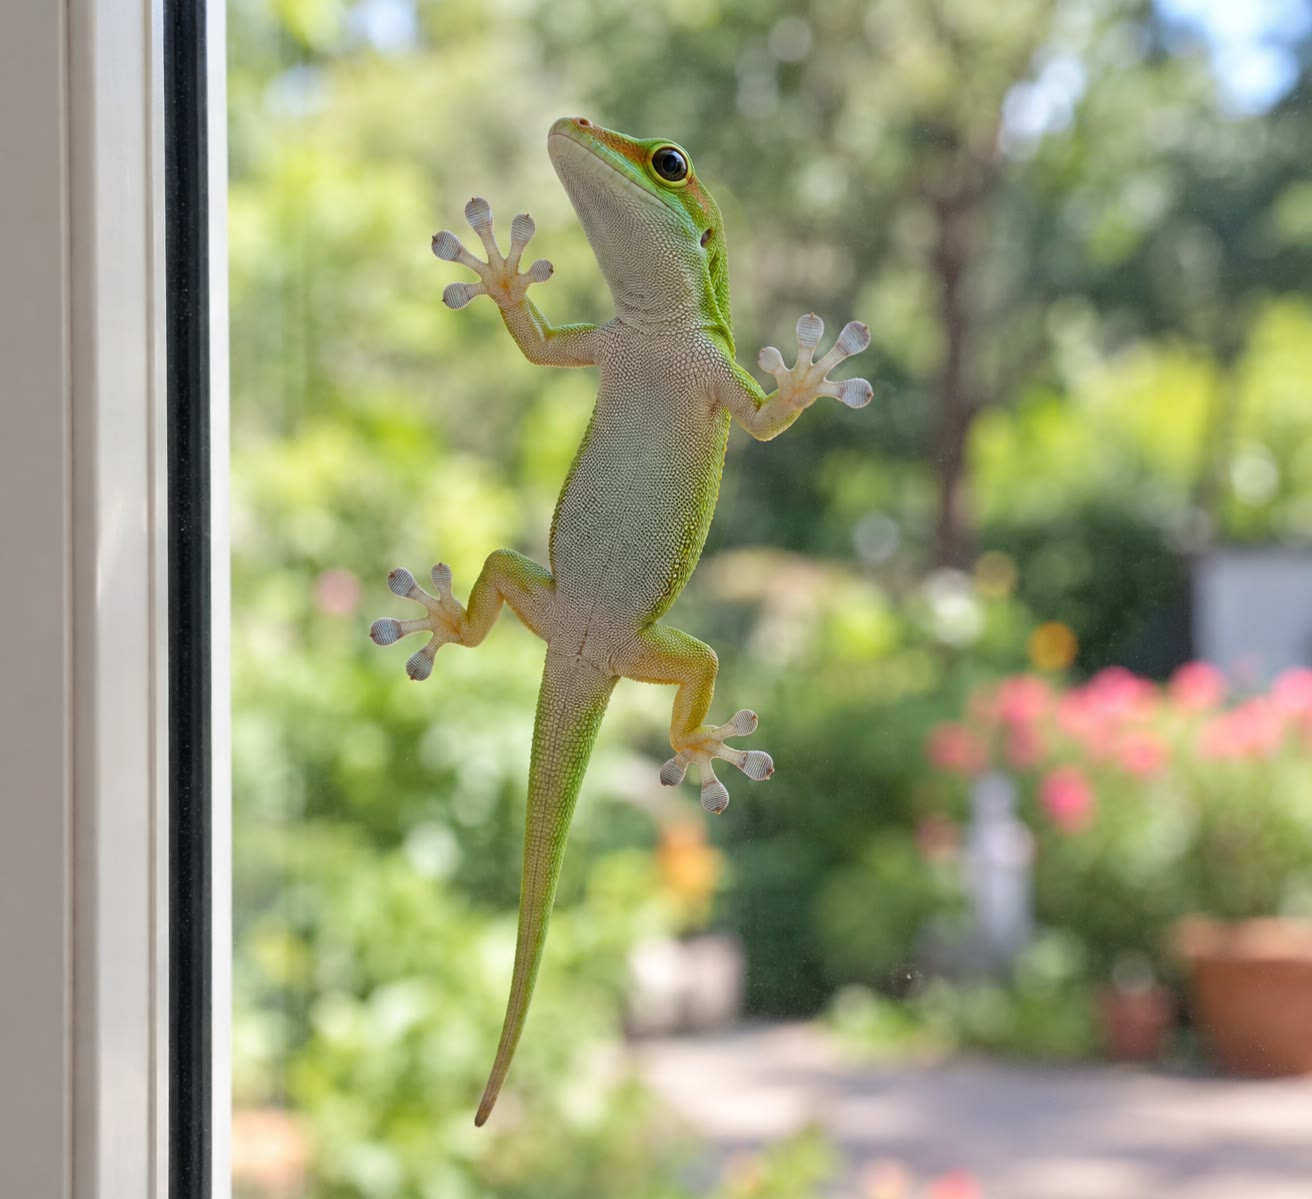
\includegraphics[width=0.52\linewidth]{images/book2/ai/b1-04-gecko.jpg}

{\small Seekor cicak pada kaca jendela. Jutaan rambut halus pada bantalan
jarinya mendekat sedemikian rapat ke kaca sehingga tarikan lemah antara
molekul-molekulnya dan molekul-molekul kaca berjumlah lebih besar
daripada beratnya.}
\end{omfigure}

\section{Interaksi van der Waals}

\begin{definition}[Interaksi van der Waals]\label{def:b1:intermolecular-forces-solvents:vdw}
\emph{Interaksi van der Waals}\index{interaksi van der Waals} adalah
gaya-gaya tarik antara molekul-molekul netral yang berasal dari interaksi
dipol-dipolnya. Dibedakan tiga jenis:
\begin{itemize}
  \item \emph{interaksi Keesom}\index{interaksi Keesom} (atau interaksi
        orientasi) antara dua dipol permanen, yang cenderung menyusun diri
        kepala ke ekor;
  \item \emph{interaksi Debye}\index{interaksi Debye} (atau interaksi
        induksi) antara dipol permanen dan dipol yang diimbasnya pada
        tetangga yang mudah terpolarisasi;
  \item \emph{interaksi London}\index{interaksi London} (atau interaksi
        dispersi) antara dipol-dipol sesaat yang ditimbulkan fluktuasi
        awan elektron pada dua atom atau molekul mana pun, polar atau
        tidak, dan yang saling mengimbas.
\end{itemize}
\end{definition}

\begin{omfigure}
\begin{tikzpicture}[font=\small, >={Stealth},
    mol/.style={draw=black!60, fill=#1, ellipse, minimum width=1.5cm, minimum height=0.8cm}]
  % Keesom
  \node[mol=omDef!20] (a) at (0,0) {}; \node[mol=omDef!20] (b) at (1.7,0) {};
  \node at (-0.45,0) {$\delta^-$}; \node at (0.45,0) {$\delta^+$};
  \node at (1.25,0) {$\delta^-$}; \node at (2.15,0) {$\delta^+$};
  \node[below, align=center] at (0.85,-0.65) {Keesom:\\dua dipol permanen};
  % Debye
  \begin{scope}[xshift=4.6cm]
    \node[mol=omDef!20] at (0,0) {}; \node[mol=black!5, dashed] at (1.7,0) {};
    \node at (-0.45,0) {$\delta^-$}; \node at (0.45,0) {$\delta^+$};
    \node[omProp] at (1.25,0) {$\delta^-$}; \node[omProp] at (2.15,0) {$\delta^+$};
    \node[below, align=center] at (0.85,-0.65) {Debye:\\permanen dan imbas};
  \end{scope}
  % London
  \begin{scope}[xshift=9.2cm]
    \node[mol=black!5, dashed] at (0,0) {}; \node[mol=black!5, dashed] at (1.7,0) {};
    \node[omProp] at (-0.45,0) {$\delta^-$}; \node[omProp] at (0.45,0) {$\delta^+$};
    \node[omProp] at (1.25,0) {$\delta^-$}; \node[omProp] at (2.15,0) {$\delta^+$};
    \node[below, align=center] at (0.85,-0.65) {London:\\dua dipol sesaat};
  \end{scope}
\end{tikzpicture}

{\small Tiga \omterm{def:b1:intermolecular-forces-solvents:vdw}{interaksi van der Waals}. Muatan parsial hitam bersifat
permanen (\omterm{def:b1:lewis-resonance-vsepr:dipole}{molekul polar}); yang jingga bersifat imbas atau sesaat. Dalam
setiap kasus muatan-muatan yang berhadapan berlawanan tanda, sehingga
molekul-molekulnya saling tarik.}
\end{omfigure}

\begin{proposition}[Kekuatan dan jangkauan]\label{prop:b1:intermolecular-forces-solvents:distance-law}
Untuk dua molekul yang berjarak $r$, masing-masing ketiga energi van der
Waals berubah sebanding dengan $-1/r^6$: tarikannya hanya terasa antara
tetangga dekat. Energinya berorde beberapa kilojoule per mol, sekitar
seratus kali lebih kecil daripada \omterm{def:b1:lewis-resonance-vsepr:lewis}{ikatan kovalen}. Suku London membesar
dengan \omterm{def:b1:periodicity:polarisability}{polarisabilitas} kedua pihak; suku ini ada di antara semua molekul
dan biasanya yang terbesar di antara ketiganya, kecuali untuk molekul
kecil yang sangat polar.
\end{proposition}
\admitted

\begin{example}[Gas mulia dan halogen]\label{ex:b1:intermolecular-forces-solvents:noble}
Atom-atom gas mulia saling tarik hanya melalui gaya London, yang membesar
dengan banyaknya elektron: helium mendidih pada \qty{-268.9}{\celsius},
neon pada \qty{-246.1}{\celsius}, argon pada \qty{-185.9}{\celsius},
kripton pada \qty{-153.4}{\celsius}, xenon pada \qty{-108.1}{\celsius}.
Demikian pula, pada suhu kamar difluorin dan diklor berwujud gas, dibrom
cair (mendidih pada \qty{58.8}{\celsius}), dan diiodin padat.
% ledger: bp:He, bp:Ne, bp:Ar, bp:Kr, bp:Xe, bp:F2, bp:Cl2, bp:Br2, bp:I2
\end{example}

\begin{omfigure}
\begin{tikzpicture}
\begin{axis}[
  width=0.62\linewidth, height=5.4cm,
  xmin=0.5, xmax=10.5, ymin=-180, ymax=200,
  axis x line=bottom, axis y line=left,
  xlabel={banyaknya atom karbon $n$}, ylabel={titik didih (\unit{\celsius})},
  xtick={1,2,3,4,5,6,7,8,9,10}, ytick={-150,-100,-50,0,50,100,150},
  tick label style={font=\small}, label style={font=\small}]
\addplot[omDef, thick, mark=*, mark size=1.5pt] table[x=n, y=bp_C] {figdata/out/bachelor-1-hydride-boiling-points-alkanes.dat};
\end{axis}
\end{tikzpicture}

{\small Titik didih alkana rantai lurus \ce{C_nH_{2n+2}}, dari metana
sampai dekana. Setiap \ce{CH2} yang ditambahkan menambah elektron dan
luas permukaan kontak, sehingga menambah tarikan London; pertambahannya
mengecil perlahan, dari sekitar \qty{75}{\celsius} pada awalnya menjadi
\qty{25}{\celsius} pada dekana.}
\end{omfigure}

\section{Ikatan hidrogen}

\begin{definition}[Ikatan hidrogen]\label{def:b1:intermolecular-forces-solvents:hbond}
\emph{Ikatan hidrogen}\index{ikatan hidrogen} adalah tarikan
$\ce{X-H}\cdots\ce{Y}$ antara atom hidrogen yang terikat pada atom X yang
kecil dan sangat elektronegatif (\ce{N}, \ce{O}, atau \ce{F}) dan
\omterm{def:b1:lewis-resonance-vsepr:lewis}{sepasang elektron bebas} atom elektronegatif lain Y. Molekul yang membawa
\ce{X-H} adalah donor ikatan hidrogen, molekul yang membawa Y
akseptornya. Energinya, 10 sampai \qty{40}{kJ/mol}, terletak di antara
energi \omterm{def:b1:intermolecular-forces-solvents:vdw}{interaksi van der Waals} dan energi \omterm{def:b1:lewis-resonance-vsepr:lewis}{ikatan kovalen}; ketiga atom
\ce{X}, \ce{H}, \ce{Y} hampir segaris.
\end{definition}

\begin{remark}[Mengapa N, O, dan F]\label{rem:b1:intermolecular-forces-solvents:why}
Atom X yang sangat elektronegatif meninggalkan muatan parsial positif
yang besar pada hidrogen; hidrogen, yang tidak mempunyai elektron dalam,
sangat kecil, sehingga \omterm{def:b1:lewis-resonance-vsepr:lewis}{pasangan elektron bebas} Y dapat mendekatinya
sangat rapat. Kedua syarat itu diperlukan: ikatan \ce{C-H} kurang polar,
sedangkan ikatan \ce{S-H} atau \ce{Cl-H} melibatkan atom-atom yang
terlalu besar dan terlalu lemah \omterm{def:b1:periodicity:electronegativity}{keelektronegatifannya} untuk membentuk
\omterm{def:b1:intermolecular-forces-solvents:hbond}{ikatan hidrogen} yang kuat.
\end{remark}

\begin{omfigure}
\begin{tikzpicture}[font=\small]
  % water network
  \foreach \n/\x/\y/\a in {1/0/0/0, 2/2.2/0.9/200, 3/0.2/-2.0/60, 4/-2.1/0.6/-30} {
    \begin{scope}[shift={(\x,\y)}, rotate=\a]
      \node[aO] (o\n) at (0,0) {};
      \node[aH] (h\n a) at (0.78,0.3) {};
      \node[aH] (h\n b) at (-0.2,-0.82) {};
      \begin{scope}[on background layer]
        \draw[bond] (o\n.center) -- (h\n a.center); \draw[bond] (o\n.center) -- (h\n b.center);
      \end{scope}
    \end{scope}
  }
  \draw[omThm, thick, densely dotted] (h1a) -- (o2);
  \draw[omThm, thick, densely dotted] (h1b) -- (o3);
  \draw[omThm, thick, densely dotted] (h4a) -- (o1);
  \node[below, align=center] at (0,-2.9) {air: setiap molekul dapat\\memberi dua dan menerima dua};
  % carboxylic acid dimer
  \begin{scope}[xshift=5.6cm, yshift=-0.6cm]
    \node (r1) at (-0.9,0) {R}; \node (c1) at (0,0) {C};
    \node (o1) at (0.6,0.85) {O}; \node (o2) at (0.6,-0.85) {O}; \node (h2) at (1.45,-0.85) {H};
    \node (c2) at (3.3,0) {C}; \node (r2) at (4.2,0) {R};
    \node (o3) at (2.7,0.85) {O}; \node (o4) at (2.7,-0.85) {O}; \node (h3) at (1.85,0.85) {H};
    \draw (r1) -- (c1) -- (o2) -- (h2) (c2) -- (r2) (c2) -- (o3) -- (h3);
    \draw[double, double distance=1.6pt] (c1) -- (o1); \draw[double, double distance=1.6pt] (c2) -- (o4);
    \draw[omThm, thick, densely dotted] (h2) -- (o4) (h3) -- (o1);
    \node[below] at (1.65,-2.3) {dimer asam karboksilat};
  \end{scope}
\end{tikzpicture}

{\small \omterm{def:b1:intermolecular-forces-solvents:hbond}{Ikatan hidrogen} (titik-titik merah). Dalam air cair setiap
molekul terlibat dalam paling banyak empat \omterm{def:b1:intermolecular-forces-solvents:hbond}{ikatan hidrogen}; asam
karboksilat berpasangan menjadi dimer siklik yang diikat oleh dua \omterm{def:b1:intermolecular-forces-solvents:hbond}{ikatan
hidrogen}.}
\end{omfigure}

\begin{proposition}[Ikatan hidrogen menaikkan titik didih]\label{prop:b1:intermolecular-forces-solvents:hbond-bp}
Di antara hidrida \omterm{def:b1:periodicity:table}{golongan} 15, 16, dan 17, titik didih naik dari \omterm{def:b1:periodicity:table}{periode}
3 ke \omterm{def:b1:periodicity:table}{periode} 5, mengikuti \omterm{def:b1:intermolecular-forces-solvents:vdw}{interaksi London}; hidrida \omterm{def:b1:periodicity:table}{periode} 2, \ce{NH3},
\ce{H2O}, dan \ce{HF}, yang membentuk \omterm{def:b1:intermolecular-forces-solvents:hbond}{ikatan hidrogen}, mendidih jauh di
atas ekstrapolasi kecenderungan itu. Hidrida \omterm{def:b1:periodicity:table}{golongan} 14 (\ce{CH4},
\ce{SiH4}, \ce{GeH4}) tidak membentuk \omterm{def:b1:intermolecular-forces-solvents:hbond}{ikatan hidrogen} dan mengikuti
kecenderungan tersebut.
\end{proposition}

\begin{omfigure}
\begin{tikzpicture}
\begin{axis}[
  width=0.82\linewidth, height=6.6cm,
  xmin=1.5, xmax=5.6, ymin=-180, ymax=120,
  axis x line=bottom, axis y line=left,
  xlabel={periode}, ylabel={titik didih (\unit{\celsius})},
  xtick={2,3,4,5}, ytick={-150,-100,-50,0,50,100},
  tick label style={font=\small}, label style={font=\small},
  clip=false]
\addplot[black!60, thick, mark=square*, mark size=1.6pt] table[x=period, y=bp_C] {figdata/out/bachelor-1-hydride-boiling-points-g14.dat};
\addplot[omDef, thick, mark=*, mark size=1.6pt] table[x=period, y=bp_C] {figdata/out/bachelor-1-hydride-boiling-points-g15.dat};
\addplot[omThm, thick, mark=*, mark size=1.6pt] table[x=period, y=bp_C] {figdata/out/bachelor-1-hydride-boiling-points-g16.dat};
\addplot[omMeth, thick, mark=triangle*, mark size=2pt] table[x=period, y=bp_C] {figdata/out/bachelor-1-hydride-boiling-points-g17.dat};
\addplot[omThm, dashed] coordinates {(2,-79.3) (3,-60.3)};
\node[font=\small, anchor=west] at (axis cs:2.05,100) {\ce{H2O}};
\node[font=\small, anchor=west] at (axis cs:2.05,19.6) {\ce{HF}};
\node[font=\small, anchor=west] at (axis cs:2.05,-30) {\ce{NH3}};
\node[font=\small, anchor=east] at (axis cs:1.96,-162) {\ce{CH4}};
\node[font=\small, anchor=west] at (axis cs:4.05,-41.3) {\ce{H2Se}};
\node[font=\small, anchor=west] at (axis cs:5.05,-18.4) {\ce{SbH3}};
\node[font=\small, anchor=west] at (axis cs:5.05,-35.1) {\ce{HI}};
\node[font=\small, anchor=west] at (axis cs:4.05,-88.1) {\ce{GeH4}};
\node[font=\small, omThm, anchor=north west] at (axis cs:2.05,-85) {ekstrapolasi};
\end{axis}
\end{tikzpicture}

{\small Titik didih hidrida \omterm{def:b1:periodicity:table}{golongan} 14 (bujur sangkar abu-abu), 15
(biru), 16 (merah), dan 17 (hijau). Air akan mendidih di dekat
\qty{-79}{\celsius} seandainya mengikuti analog-analognya yang lebih
berat (garis putus-putus); \omterm{def:b1:intermolecular-forces-solvents:hbond}{ikatan hidrogennya} menaikkan titik didih itu
sekitar \qty{180}{\celsius}.}
% ledger: bp:CH4, bp:SiH4, bp:GeH4, bp:NH3, bp:PH3, bp:AsH3, bp:SbH3,
% bp:H2O, bp:H2S, bp:H2Se, bp:HF, bp:HCl, bp:HBr, bp:HI
\end{omfigure}

\begin{example}[Etanol dan isomernya]\label{ex:b1:intermolecular-forces-solvents:isomers}
Etanol, \ce{CH3CH2OH}, dan metoksimetana, \ce{CH3OCH3}, mempunyai rumus
yang sama, \ce{C2H6O}, dan \omterm{def:b1:intermolecular-forces-solvents:vdw}{interaksi London} yang hampir sama. Etanol,
yang gugus \ce{O-H}-nya sekaligus donor dan akseptor, mendidih pada
\qty{78.4}{\celsius}; metoksimetana, yang hanya dapat menerima, mendidih
pada \qty{-25.0}{\celsius}.
% ledger: bp:C2H5OH, bp:CH3OCH3
\end{example}

\section{Pelarut}

\begin{definition}[Permitivitas relatif]\label{def:b1:intermolecular-forces-solvents:permittivity}
Di dalam suatu medium, gaya Coulomb antara dua muatan dibagi dengan
bilangan $\varepsilon_r \ge 1$, yaitu \emph{permitivitas
relatif}\index{permitivitas relatif} (atau tetapan dielektrik) medium
itu:
\[
  F = \frac{|q_1 q_2|}{4\pi\varepsilon_0\varepsilon_r r^2} .
\]
Nilainya besar untuk zat cair yang molekulnya polar, yang mengorientasikan
diri di sekitar muatan-muatan dan menapisnya: \num{78.4} untuk air pada
\qty{25}{\celsius}, \num{1.89} untuk heksana pada \qty{20}{\celsius}.
% ledger: epsr:H2O, epsr:C6H14
\end{definition}

\begin{definition}[Pelarut polar, protik, dan aprotik]\label{def:b1:intermolecular-forces-solvents:solvent-classes}
\emph{Pelarut polar}\index{pelarut polar} terdiri atas molekul-molekul
dengan \omterm{def:b1:lewis-resonance-vsepr:dipole}{momen dipol} besar dan mempunyai \omterm{def:b1:intermolecular-forces-solvents:permittivity}{permitivitas relatif} yang besar
(di atas sekitar 15); pelarut apolar mempunyai permitivitas yang kecil.
\emph{Pelarut protik}\index{pelarut protik} mempunyai molekul-molekul
yang membawa atom hidrogen yang mampu membentuk \omterm{def:b1:intermolecular-forces-solvents:hbond}{ikatan hidrogen}
(\ce{O-H} atau \ce{N-H}); \emph{pelarut aprotik}\index{pelarut aprotik}
tidak mempunyainya.
\end{definition}

\begin{center}
\small
\begin{tabular}{lccll}
\hline
pelarut & $\varepsilon_r$ & $\mu$ (D) & kepolaran & keprotikan \\
\hline
air & 78.4 & 1.86 & polar & protik \\
metanol & 32.6 & 1.67 & polar & protik \\
etanol & 24.3 & 1.52 & polar & protik \\
asetonitril, \ce{CH3CN} & 37.5 & 3.92 & polar & aprotik \\
propanon (aseton) & 20.7 & 2.88 & polar & aprotik \\
diklorometana & 9.08 & 1.62 & agak polar & aprotik \\
etil etanoat & 6.02 & 1.78 & agak polar & aprotik \\
etoksietana & 4.34 & 1.15 & agak polar & aprotik \\
benzena & 2.28 & 0 & apolar & aprotik \\
heksana & 1.89 & 0 & apolar & aprotik \\
\hline
\end{tabular}
\end{center}
% ledger: epsr:H2O, epsr:CH3OH, epsr:C2H5OH, epsr:CH3CN, epsr:CH3COCH3,
% epsr:CH2Cl2, epsr:EtOAc, epsr:Et2O, epsr:C6H6, epsr:C6H14, dip:H2O,
% dip:CH3OH, dip:C2H5OH, dip:CH3CN, dip:CH3COCH3, dip:CH2Cl2, dip:EtOAc,
% dip:Et2O, dip:C6H6 (relative permittivities at 20 or 25 degC; dipole
% moments of the gas-phase molecules; hexane has no dipole by symmetry)

\begin{definition}[Solvasi, daya pengion, dan daya disosiasi]\label{def:b1:intermolecular-forces-solvents:dissolution}
\emph{Solvasi}\index{solvasi} sebuah partikel zat terlarut adalah
pengelilingannya oleh molekul-molekul pelarut yang terorientasi dan
terikat padanya oleh gaya-gaya antarmolekul (hidrasi, di dalam air).
\emph{Daya pengion}\index{daya pengion} sebuah pelarut adalah
kemampuannya mengubah \omterm{def:b1:lewis-resonance-vsepr:lewis}{ikatan kovalen} polar zat terlarut menjadi pasangan
ion, sifat \omterm{def:b1:intermolecular-forces-solvents:solvent-classes}{pelarut polar} dengan \omterm{def:b1:lewis-resonance-vsepr:dipole}{momen dipol} yang besar; \emph{daya
disosiasi}\index{daya disosiasi} pelarut itu adalah kemampuannya
memisahkan ion-ion sebuah pasangan, yang diukur dengan \omterm{def:b1:intermolecular-forces-solvents:permittivity}{permitivitas
relatifnya}.
\end{definition}

\begin{proposition}[Pelarutan dalam tiga tahap]\label{prop:b1:intermolecular-forces-solvents:steps}
Pelarutan sebuah elektrolit di dalam pelarut dapat dipaparkan dalam tiga
tahap: ionisasi (untuk zat terlarut molekuler seperti \ce{HCl}),
disosiasi pasangan-pasangan ion, dan \omterm{def:b1:intermolecular-forces-solvents:dissolution}{solvasi} ion-ion yang terpisah.
Sebuah pelarut melarutkan zat terlarut ionik atau sangat polar dengan
baik jika pelarut itu polar (mengionkan), berpermitivitas tinggi
(mendisosiasikan), dan mampu menyolvasi kedua ion --- kation melalui
\omterm{def:b1:lewis-resonance-vsepr:lewis}{pasangan elektron bebasnya}, anion melalui \omterm{def:b1:intermolecular-forces-solvents:hbond}{ikatan hidrogen} jika pelarut
itu protik. Air melakukan ketiganya.
\end{proposition}

\begin{example}[Hidrogen klorida dalam air dan dalam heksana]\label{ex:b1:intermolecular-forces-solvents:hcl}
Dalam air, \ce{HCl} terionisasi dan terdisosiasi sempurna:
\ce{HCl(g) + H2O(l) -> H3O+(aq) + Cl-(aq)}; larutannya menghantarkan
listrik. Dalam heksana, yang apolar dan berpermitivitas rendah, zat itu
larut sebagai molekul \ce{HCl} dan larutannya tidak menghantarkan
listrik.
\end{example}

\begin{omfigure}
\begin{tikzpicture}[font=\small]
  \node[aNa] (na) at (0,0) {};
  \node[font=\scriptsize, white] at (na) {\ce{Na+}};
  \foreach \a in {0,60,...,300} {
    \begin{scope}[shift={(\a:1.25)}, rotate=\a]
      \node[aO] (o) at (0,0) {};
      \node[aH] (ha) at (0.55,0.5) {}; \node[aH] (hb) at (0.55,-0.5) {};
      \begin{scope}[on background layer]
        \draw[bond] (o.center) -- (ha.center); \draw[bond] (o.center) -- (hb.center);
      \end{scope}
    \end{scope}
  }
  \node[below, align=center] at (0,-2.4) {kation: pasangan bebas\\oksigen mengarah ke dalam};
  \begin{scope}[xshift=6.2cm]
    \node[aCl] (cl) at (0,0) {};
    \node[font=\scriptsize, white] at (cl) {\ce{Cl-}};
    \foreach \a in {0,60,...,300} {
      \begin{scope}[shift={(\a:1.55)}, rotate=\a]
        \node[aH] (h1) at (-0.62,0) {};
        \node[aO] (o) at (0,0) {};
        \node[aH] (h2) at (0.25,0.72) {};
        \begin{scope}[on background layer]
          \draw[bond] (o.center) -- (h1.center); \draw[bond] (o.center) -- (h2.center);
        \end{scope}
      \end{scope}
    }
    \node[below, align=center] at (0,-2.4) {anion: ikatan hidrogen\\mengarah ke dalam};
  \end{scope}
\end{tikzpicture}

{\small Hidrasi kedua ion natrium klorida (hanya lapisan pertama, digambar
pada bidang). Air menghadapkan ujung negatifnya, oksigen, ke kation, dan
satu hidrogennya ke anion.}
\end{omfigure}

\section{Kelarutan, sifat dapat bercampur, dan amfifil}

\begin{proposition}[Yang sejenis melarutkan yang sejenis]\label{prop:b1:intermolecular-forces-solvents:like}
Sebuah zat terlarut larut dengan baik dalam suatu pelarut jika interaksi
antara molekul-molekul zat terlarut dan pelarut sebanding dengan
interaksi yang hilang: zat terlarut polar atau pembentuk ion dalam
\omterm{def:b1:intermolecular-forces-solvents:solvent-classes}{pelarut polar}, zat terlarut apolar dalam pelarut apolar, zat terlarut
pembentuk \omterm{def:b1:intermolecular-forces-solvents:hbond}{ikatan hidrogen} dalam \omterm{def:b1:intermolecular-forces-solvents:solvent-classes}{pelarut protik}.
\end{proposition}

\begin{proof}[Penalaran]
Pelarutan memutus interaksi zat terlarut--zat terlarut dan
pelarut--pelarut serta membentuk interaksi zat terlarut--pelarut. Jika
zat terlarutnya apolar dan pelarutnya air, molekul-molekul air
kehilangan \omterm{def:b1:intermolecular-forces-solvents:hbond}{ikatan hidrogen} untuk memberi tempat baginya dan sebagai
gantinya hanya memperoleh \omterm{def:b1:intermolecular-forces-solvents:vdw}{interaksi London} yang lemah: pelarutan tidak
menguntungkan. Jika keduanya apolar, \omterm{def:b1:intermolecular-forces-solvents:vdw}{interaksi London} yang hilang dan
yang diperoleh sebanding, dan pencampuran didorong oleh
ketidakteraturan yang ditimbulkannya.
\end{proof}

\begin{definition}[Zat cair yang dapat bercampur]\label{def:b1:intermolecular-forces-solvents:miscibility}
Dua zat cair disebut \emph{dapat bercampur}\index{dapat bercampur} jika
keduanya bercampur dalam segala perbandingan menjadi satu fase cair;
jika tidak, keduanya membentuk dua lapisan, dengan yang kurang rapat di
atas.
\end{definition}

\begin{example}[Air dengan etanol, air dengan heksana]\label{ex:b1:intermolecular-forces-solvents:miscible}
Etanol \omterm{def:b1:intermolecular-forces-solvents:miscibility}{dapat bercampur} dengan air: keduanya protik dan polar, dan etanol
membentuk \omterm{def:b1:intermolecular-forces-solvents:hbond}{ikatan hidrogen} dengan air seperti halnya dengan dirinya
sendiri. Heksana dan air tidak \omterm{def:b1:intermolecular-forces-solvents:miscibility}{dapat bercampur}. Diiodin, sebuah padatan
molekuler, nyaris tidak larut dalam air, tetapi mudah larut dalam
heksana atau diklorometana: jika dikocok dengan pelarut semacam itu,
iodin dari fase berair berpindah ke lapisan organik, prinsip ekstraksi
cair--cair (\cref{ch:b1:lab-techniques-1}).
\end{example}

\begin{omfigure}
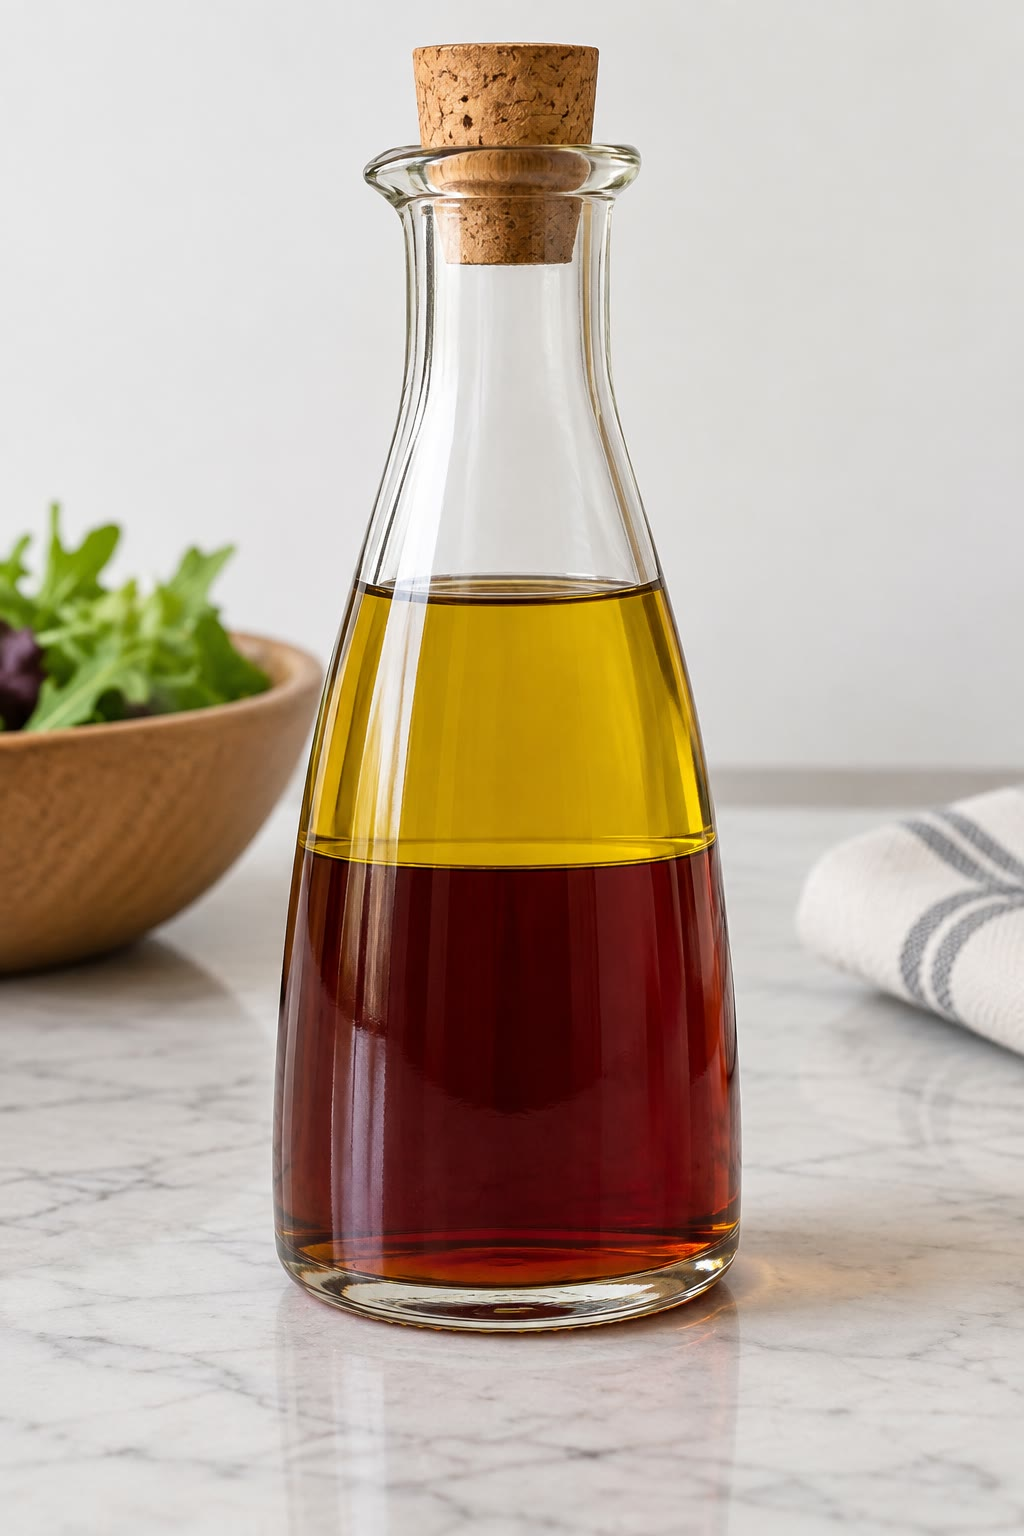
\includegraphics[width=0.2\linewidth]{images/book2/ai/b1-04-dressing.jpg}

{\small Saus salad yang didiamkan: minyak zaitun, yang apolar, mengapung
di atas cuka, sebuah larutan berair; kedua zat cair itu tidak \omterm{def:b1:intermolecular-forces-solvents:miscibility}{dapat
bercampur}.}
\end{omfigure}

\begin{definition}[Hidrofilik, hidrofobik, amfifilik]\label{def:b1:intermolecular-forces-solvents:amphiphile}
Sebuah gugus bersifat \emph{hidrofilik}\index{hidrofilik} jika berinteraksi
secara menguntungkan dengan air (gugus ionik atau polar: \ce{-COO^-},
\ce{-OH}, \ce{-SO3^-}) dan \emph{hidrofobik}\index{hidrofobik} jika tidak
(rantai hidrokarbon). Sebuah molekul bersifat
\emph{amfifilik}\index{amfifilik} jika membawa sekaligus kepala yang
hidrofilik dan ekor yang hidrofobik.
\end{definition}

\begin{example}[Sabun]\label{ex:b1:intermolecular-forces-solvents:soap}
Natrium dodekanoat, \ce{CH3(CH2)10COO- Na+}, bersifat \omterm{def:b1:intermolecular-forces-solvents:amphiphile}{amfifilik}. Di
permukaan air, molekul-molekulnya berdiri dengan kepala di dalam air dan
ekor di udara. Di bagian dalam cairan, di atas suatu konsentrasi yang
kecil, molekul-molekul itu berkumpul membentuk bola --- misel --- dengan
ekor di dalam dan kepala di luar. Lemak, yang apolar, larut dalam inti
\omterm{def:b1:intermolecular-forces-solvents:amphiphile}{hidrofobik} misel dan terbawa pergi oleh air.
\end{example}

\begin{omfigure}
\begin{tikzpicture}[font=\small]
  % interface
  \fill[omWater] (-3.2,-1.6) rectangle (-0.4,0);
  \draw[omDef!60] (-3.2,0) -- (-0.4,0);
  \node[anchor=south west] at (-3.2,0.95) {udara};
  \node[anchor=north west] at (-3.2,-1.2) {air};
  \foreach \x in {-2.9,-2.5,...,-0.6} {
    \fill[omThm] (\x,-0.12) circle (0.11);
    \draw[thick, black!70, decorate, decoration={zigzag, amplitude=1pt, segment length=3pt}] (\x,0) -- (\x,0.85);
  }
  % micelle
  \begin{scope}[xshift=3.2cm, yshift=-0.4cm]
    \fill[omWater] (-2,-1.6) rectangle (2,1.6);
    \foreach \a in {0,30,...,330} {
      \draw[thick, black!70, decorate, decoration={zigzag, amplitude=1pt, segment length=3pt}] (\a:0.25) -- (\a:1.0);
      \fill[omThm] (\a:1.12) circle (0.11);
    }
    \node[anchor=north] at (0,-1.65) {misel di dalam air};
  \end{scope}
\end{tikzpicture}

{\small Molekul-molekul \omterm{def:b1:intermolecular-forces-solvents:amphiphile}{amfifilik} (kepala \omterm{def:b1:intermolecular-forces-solvents:amphiphile}{hidrofilik} merah, ekor
\omterm{def:b1:intermolecular-forces-solvents:amphiphile}{hidrofobik} zig-zag) di permukaan air dan berkumpul menjadi misel, digambar
dalam penampang; misel dipelajari dalam jilid Tahun 3.}
\end{omfigure}

\begin{method}[Memilih pelarut]\label{met:b1:intermolecular-forces-solvents:choose}
Untuk memilih pelarut bagi sebuah zat terlarut atau sebuah reaksi:
\begin{enumerate}
  \item cirikan zat terlarutnya: ionik, polar, mampu memberi atau menerima
        \omterm{def:b1:intermolecular-forces-solvents:hbond}{ikatan hidrogen}, atau apolar;
  \item pilihlah pelarut yang sejenis (\cref{prop:b1:intermolecular-forces-solvents:like}),
        yang permitivitasnya tinggi jika ion-ion harus dipisahkan;
  \item untuk reaksi antara anion dan molekul, utamakan \omterm{def:b1:intermolecular-forces-solvents:solvent-classes}{pelarut polar}
        aprotik, yang melarutkan garamnya tanpa mengikat anion melalui
        \omterm{def:b1:intermolecular-forces-solvents:hbond}{ikatan hidrogen} (\cref{ch:b1:nucleophilic-substitution});
  \item untuk ekstraksi, pilihlah pelarut yang tidak \omterm{def:b1:intermolecular-forces-solvents:miscibility}{dapat bercampur}
        dengan pelarut pertama dan yang jauh lebih banyak melarutkan zat
        terlarutnya.
\end{enumerate}
\end{method}

\section{Latihan}

\begin{exercise}[$\star$]\label{exo:b1:intermolecular-forces-solvents:1}
Sebutkan interaksi yang ada di antara partikel-partikel argon cair,
hidrogen klorida cair, air cair, metana cair, dan diiodin padat, lalu
nyatakan interaksi mana yang dominan pada masing-masing.
\end{exercise}

\begin{exercise}[$\star$]\label{exo:b1:intermolecular-forces-solvents:2}
Manakah di antara zat-zat berikut yang membentuk \omterm{def:b1:intermolecular-forces-solvents:hbond}{ikatan hidrogen} di
antara molekul-molekulnya sendiri: \ce{CH3OH}, \ce{CH3OCH3},
\ce{CH3NH2}, \ce{CH3F}, \ce{HF}, \ce{CH4}? Manakah yang hanya dapat
menerima \omterm{def:b1:intermolecular-forces-solvents:hbond}{ikatan hidrogen} dari molekul lain?
\end{exercise}

\begin{exercise}[$\star$]\label{exo:b1:intermolecular-forces-solvents:3}
Dengan tabel pelarut, golongkan air, etanol, propanon, heksana,
diklorometana, dan asetonitril sebagai polar atau apolar, protik atau
aprotik.
\end{exercise}

\begin{exercise}[$\star$]\label{exo:b1:intermolecular-forces-solvents:4}
Jelaskan mengapa diiodin jauh lebih mudah larut dalam heksana daripada
dalam air, dan mengapa natrium klorida justru sebaliknya.
\end{exercise}

\begin{exercise}[$\star\star$]\label{exo:b1:intermolecular-forces-solvents:5}
Metanol mendidih pada \qty{64.7}{\celsius}, etanol pada
\qty{78.4}{\celsius}, asam etanoat pada \qty{118.1}{\celsius}, dan
metoksimetana pada \qty{-25.0}{\celsius}. Jelaskan urutan itu.
% ledger: bp:CH3OH, bp:C2H5OH, bp:CH3COOH, bp:CH3OCH3
\end{exercise}

\begin{exercise}[$\star\star$]\label{exo:b1:intermolecular-forces-solvents:6}
Hitunglah gaya Coulomb antara ion \ce{Na+} dan ion \ce{Cl-} yang
berjarak \qty{500}{pm} di vakum ($\varepsilon_0 = \qty{8.854e-12}{F/m}$,
$e = \qty{1.602e-19}{C}$), lalu di dalam air ($\varepsilon_r = 78.4$) dan
di dalam heksana ($\varepsilon_r = 1.89$). Berikan komentar.
\end{exercise}

\begin{exercise}[$\star\star$]\label{exo:b1:intermolecular-forces-solvents:7}
Propanon dan air \omterm{def:b1:intermolecular-forces-solvents:miscibility}{dapat bercampur} dalam segala perbandingan; heksana dan
air tidak. Jelaskan, dengan memperhatikan interaksi yang diputus dan yang
dibentuk.
\end{exercise}

\begin{exercise}[$\star\star$]\label{exo:b1:intermolecular-forces-solvents:8}
\ce{HCl} mempunyai \omterm{def:b1:lewis-resonance-vsepr:dipole}{momen dipol} \qty{1.09}{\debye} dan mendidih pada
\qty{-85.0}{\celsius}; \ce{HBr} mempunyai \qty{0.83}{\debye} dan mendidih
pada \qty{-66.4}{\celsius}. Mengapa molekul yang kurang polar mendidih
pada suhu yang lebih tinggi?
% ledger: dip:HCl, dip:HBr, bp:HCl, bp:HBr
\end{exercise}

\begin{exercise}[$\star\star$]\label{exo:b1:intermolecular-forces-solvents:9}
Gambarlah dimer siklik asam etanoat. Dalam larutan benzena, asam etanoat
berperilaku seakan-akan massa molarnya sekitar dua kali \qty{60}{g/mol};
dalam air tidak demikian. Jelaskan kedua fakta itu.
\end{exercise}

\begin{exercise}[$\star\star\star$]\label{exo:b1:intermolecular-forces-solvents:10}
Paparkan pelarutan natrium klorida dalam air dari segi disosiasi dan
\omterm{def:b1:intermolecular-forces-solvents:dissolution}{solvasi}, dan pelarutan hidrogen klorida dalam air dari segi ionisasi,
disosiasi, dan \omterm{def:b1:intermolecular-forces-solvents:dissolution}{solvasi}. Mengapa hidrogen klorida dalam heksana
menghasilkan larutan yang tidak menghantarkan listrik?
\end{exercise}

\begin{exercise}[$\star\star\star$]\label{exo:b1:intermolecular-forces-solvents:11}
Dari titik didih alkana rantai lurus (pentana \qty{36.1}{\celsius},
dekana \qty{174.1}{\celsius}), hitunglah kenaikan rata-rata per gugus
\ce{CH2} antara \ce{C5} dan \ce{C10}, lalu perkirakan titik didih
undekana. Mengapa pertambahannya mengecil sepanjang deret itu?
% ledger: bp:C5H12, bp:C10H22
\end{exercise}

\begin{exercise}[$\star\star\star$]\label{exo:b1:intermolecular-forces-solvents:12}
Natrium dodesil sulfat, \ce{CH3(CH2)11OSO3^- Na+}, adalah sebuah
deterjen. Tentukan bagian \omterm{def:b1:intermolecular-forces-solvents:amphiphile}{hidrofilik} dan \omterm{def:b1:intermolecular-forces-solvents:amphiphile}{hidrofobiknya}, sketsalah
susunannya di permukaan air dan di dalam misel, lalu jelaskan bagaimana
zat itu menghilangkan noda berminyak dari kain.
\end{exercise}

\section{Soal: Seandainya Air Tidak Mempunyai Ikatan Hidrogen}

\begin{problem}[{Soal akhir pekan --- gaya London pada gas mulia dan
alkana, pemilihan pelarut, dan titik didih yang akan dimiliki air tanpa
ikatan hidrogen}]
\label{pb:b1:intermolecular-forces-solvents:1}
Titik didih pada \qty{1}{atm} (dalam \unit{\celsius}): \ce{He} $-268.9$,
\ce{Ne} $-246.1$, \ce{Ar} $-185.9$, \ce{Kr} $-153.4$, \ce{Xe} $-108.1$;
pentana 36.1, heksana 68.8; \ce{CH4} $-161.5$, \ce{SiH4} $-112.0$,
\ce{GeH4} $-88.1$; \ce{NH3} $-33.4$, \ce{PH3} $-87.8$, \ce{AsH3} $-62.5$;
\ce{H2O} 100.0, \ce{H2S} $-60.3$, \ce{H2Se} $-41.3$; \ce{HF} 19.6,
\ce{HCl} $-85.0$, \ce{HBr} $-66.4$.
% ledger: bp:He, bp:Ne, bp:Ar, bp:Kr, bp:Xe, bp:C5H12, bp:C6H14, bp:CH4,
% bp:SiH4, bp:GeH4, bp:NH3, bp:PH3, bp:AsH3, bp:H2O, bp:H2S, bp:H2Se,
% bp:HF, bp:HCl, bp:HBr

\medskip
\noindent\textbf{Bagian I --- Hanya London.}
\begin{enumerate}
  \item Interaksi apakah yang mengikat atom-atom argon cair?
  \item Jelaskan kenaikan titik didih dari helium sampai xenon.
  \item Mengapa titik didih helium paling rendah di antara semua zat?
  \item Bandingkan pentana dan heksana: apa yang ditambahkan oleh satu
        gugus \ce{CH2}?
  \item Metana, silana, dan germana tidak mempunyai \omterm{def:b1:lewis-resonance-vsepr:dipole}{momen dipol}.
        Interaksi apakah yang menjelaskan urutan titik didihnya?
  \item Mengapa tidak mungkin ada \omterm{def:b1:intermolecular-forces-solvents:hbond}{ikatan hidrogen} dalam metana?
\end{enumerate}

\medskip
\noindent\textbf{Bagian II --- Memilih pelarut.}
Gunakan tabel pelarut dalam bab ini.
\begin{enumerate}[resume]
  \item Pelarut manakah dalam tabel itu yang paling baik melarutkan
        natrium klorida, dan mengapa?
  \item Dengan faktor berapakah tarikan antara dua ion lebih kecil di
        dalam air daripada di dalam heksana pada jarak yang sama?
  \item Sebuah reaksi antara anion \ce{CN-} dan sebuah molekul organik
        harus dijalankan dalam pelarut yang melarutkan garamnya tetapi
        tidak mengikat anion itu melalui \omterm{def:b1:intermolecular-forces-solvents:hbond}{ikatan hidrogen}. Pilihlah satu.
  \item Untuk mengekstraksi diiodin dari larutan berair, pelarut manakah
        dalam tabel yang akan dipilih, dan di lapisan manakah iodin akan
        berakhir?
  \item Jelaskan mengapa etanol tidak dapat dipakai untuk ekstraksi itu.
  \item Etoksietana hampir tidak \omterm{def:b1:intermolecular-forces-solvents:miscibility}{dapat bercampur} dengan air walaupun
        bersifat polar. Kemukakan sebuah penjelasan.
\end{enumerate}

\medskip
\noindent\textbf{Bagian III --- Hidrida-hidrida lainnya.}
\begin{enumerate}[resume]
  \item Untuk \omterm{def:b1:periodicity:table}{golongan} 17, hitunglah perubahan titik didih dari \ce{HCl}
        ke \ce{HBr}, lalu ekstrapolasikan perubahan yang sama mundur ke
        \omterm{def:b1:periodicity:table}{periode} 2.
  \item Bandingkan nilai ekstrapolasi itu dengan titik didih \ce{HF}.
  \item Dua pertanyaan yang sama untuk \omterm{def:b1:periodicity:table}{golongan} 15 (\ce{PH3}, \ce{AsH3},
        dan \ce{NH3}).
  \item Untuk \omterm{def:b1:periodicity:table}{golongan} 14, apakah \ce{CH4} terletak di atas atau di bawah
        ekstrapolasi dari \ce{SiH4} dan \ce{GeH4}? Mengapa hal itu tidak
        mengherankan?
  \item Urutkan kelebihan \ce{NH3}, \ce{HF}, dan air.
  \item Hitunglah \omterm{def:b1:intermolecular-forces-solvents:hbond}{ikatan hidrogen} yang dapat diberikan dan diterima oleh
        setiap molekul \ce{NH3}, \ce{HF}, dan \ce{H2O}, lalu jelaskan
        urutan itu.
\end{enumerate}

\medskip
\noindent\textbf{Bagian IV --- Air tanpa \omterm{def:b1:intermolecular-forces-solvents:hbond}{ikatan hidrogen}.}
\begin{enumerate}[resume]
  \item Mengapa \ce{H2S} dan \ce{H2Se} cocok untuk ekstrapolasi, dan
        mengapa air sendiri tidak?
  \item Hitunglah perubahan titik didih dari \ce{H2S} ke \ce{H2Se}.
  \item Tuliskan persamaan garis lurus yang melalui kedua titik ini,
        dengan \omterm{def:b1:periodicity:table}{periode} $p$ sebagai variabel.
  \item Turunkan titik didih yang akan dimiliki air pada $p = 2$.
  \item Seberapa besar \omterm{def:b1:intermolecular-forces-solvents:hbond}{ikatan hidrogen} menaikkan titik didih air?
  \item Simpulkan: pada suhu berapakah air akan mendidih seandainya
        molekul-molekulnya saling tarik seperti molekul-molekul \ce{H2S}?
\end{enumerate}
\end{problem}
